\documentclass[tikz,border=8pt]{standalone}
\usepackage[utf8]{inputenc}
\usepackage{amsmath,amssymb}
\usepackage{microtype}
\usetikzlibrary{arrows.meta, calc, positioning,
  decorations.pathmorphing, decorations.markings,
  shapes.geometric, patterns}

\definecolor{deepblue}{RGB}{122, 36, 53}
\definecolor{lightblue}{RGB}{234,215,218}
\definecolor{warmgold}{RGB}{154,106,31}
\definecolor{softgreen}{RGB}{124,95,88}
\definecolor{manifoldcolor}{RGB}{248,232,204}
\definecolor{distcolor}{RGB}{246,235,220}
\definecolor{midblue}{RGB}{138,90,50}

\tikzset{
  >=Stealth,
  mapsto/.style={->, line width=1.3pt, deepblue},
  pullbackarrow/.style={->, line width=1.2pt, warmgold},
  dfstyle/.style={->, line width=0.9pt, midblue, dashed},
  tanvec/.style={->, line width=1.5pt},
  mbox/.style={fill=manifoldcolor, draw=deepblue!40,
               line width=0.8pt, rounded corners=5pt, inner sep=8pt},
  pbox/.style={fill=distcolor, draw=softgreen!50,
               line width=0.8pt, rounded corners=5pt, inner sep=8pt},
}
\begin{document}
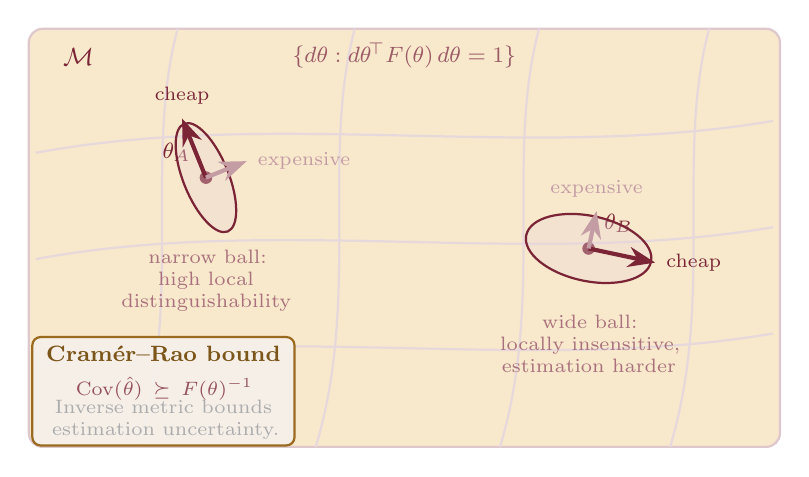
\begin{tikzpicture}[font=\small, scale=0.90]
  \fill[manifoldcolor, rounded corners=5pt]
    (-5.3,-3.1) rectangle (5.3,2.8);
  \draw[deepblue!25, rounded corners=5pt, thick]
    (-5.3,-3.1) rectangle (5.3,2.8);
  \foreach \ya in {-1.7,-0.2,1.3}{
    \draw[deepblue!18,thick]
      (-5.2,\ya-0.25) .. controls (-1.8,\ya+0.38)
                      and (1.8,\ya-0.38) .. (5.2,\ya+0.2);
  }
  \foreach \xa in {-3.4,-0.9,1.7,4.1}{
    \draw[deepblue!18,thick]
      (\xa-0.35,-3.1) .. controls (\xa+0.28,-1.0)
                      and (\xa-0.28,1.0) .. (\xa+0.2,2.8);
  }
  \node[deepblue,font=\small\bfseries] at (-4.6,2.4) {$\mathcal{M}$};
 
  % Point A: narrow ellipse
  \coordinate (ptA) at (-2.8, 0.7);
  \filldraw[deepblue] (ptA) circle (2.3pt);
  \node[deepblue,above left=3pt,font=\footnotesize\bfseries]
    at (ptA) {$\theta_A$};
  \draw[deepblue,thick,fill=lightblue,fill opacity=0.35,
        rotate around={22:(ptA)}]
    (ptA) ellipse (0.32cm and 0.82cm);
  \draw[tanvec,deepblue,rotate around={22:(ptA)}]
    (ptA) -- ++(0, 0.90)
    node[above,font=\scriptsize,yshift=1pt] {cheap};
  \draw[tanvec,deepblue!45,rotate around={22:(ptA)}]
    (ptA) -- ++(0.62, 0)
    node[right,font=\scriptsize] {expensive};
  \node[deepblue!65,font=\scriptsize,align=center,text width=2.5cm]
    at (-2.8,-0.75)
    {narrow ball:\\high local\\distinguishability};
 
  % Point B: wide ellipse
  \coordinate (ptB) at (2.6,-0.3);
  \filldraw[deepblue] (ptB) circle (2.3pt);
  \node[deepblue,above right=3pt,font=\footnotesize\bfseries]
    at (ptB) {$\theta_B$};
  \draw[deepblue,thick,fill=lightblue,fill opacity=0.35,
        rotate around={-12:(ptB)}]
    (ptB) ellipse (0.90cm and 0.46cm);
  % "cheap" now correctly along the LONG axis (0.90cm)
  \draw[tanvec,deepblue,rotate around={-12:(ptB)}]
    (ptB) -- ++(0.96, 0)
    node[right,font=\scriptsize] {cheap};
  % "expensive" now correctly along the SHORT axis (0.46cm)
  \draw[tanvec,deepblue!45,rotate around={-12:(ptB)}]
    (ptB) -- ++(0, 0.54)
    node[above,font=\scriptsize,yshift=1pt] {expensive};
  \node[deepblue!65,font=\scriptsize,align=center,text width=2.5cm]
    at (2.6,-1.65)
    {wide ball:\\locally insensitive,\\estimation harder};
 
  % Unit ball label
  \node[deepblue!75,font=\footnotesize,align=center]
    at (0, 2.42)
    {$\{d\theta:d\theta^{\!\top}F(\theta)\,d\theta=1\}$};
 
  % Cramer-Rao inset — left side
  \draw[warmgold,thick,rounded corners=3pt,
        fill=warmgold!10,fill opacity=0.97]
    (-5.25,-3.08) rectangle (-1.55,-1.55);
  \node[warmgold!80!black,font=\footnotesize\bfseries]
    at (-3.40,-1.78) {Cram\'{e}r--Rao bound};
  \node[font=\scriptsize,align=center,text width=3.0cm,deepblue!80]
    at (-3.40,-2.28)
    {$\mathrm{Cov}(\hat\theta)\succeq F(\theta)^{-1}$};
  \node[font=\scriptsize,align=center,text width=3.0cm,gray!65]
    at (-3.40,-2.72)
    {Inverse metric bounds\\estimation uncertainty.};
 
\end{tikzpicture}
\end{document}
